\documentclass[a4paper,12pt]{report}

\usepackage{alltt, fancyvrb, url}
\usepackage{graphicx}
\usepackage[utf8]{inputenc}
\usepackage{float}
\usepackage{hyperref}
\usepackage{listings}
\usepackage{xcolor}

% Questo commentalo se vuoi scrivere in inglese.
\usepackage[italian]{babel}

\usepackage[italian]{cleveref}

% Definizione stili per blocchi di codice
\lstdefinelanguage{bash}{
    keywords={cd, ls, mv, cp, rm, mkdir, rmdir, echo, cat, sudo, git, python3, pip, docker, npm},
    sensitive=true,
    morecomment=[l]{\#},
    alsoletter={-}
}
\lstdefinestyle{bash}{
    language=bash,
    basicstyle=\ttfamily\small,
    backgroundcolor=\color{gray!10},
    frame=single,
    breaklines=true,
    keywordstyle=\color{blue},
    commentstyle=\color{gray}\itshape,
}
\lstdefinestyle{java}{
    language=Java,
    basicstyle=\ttfamily\small,
    backgroundcolor=\color{gray!10},
    frame=single,
    breaklines=true,
    keywordstyle=\color{blue},
    commentstyle=\color{gray}\itshape,
    stringstyle=\color{orange},
}
\lstdefinestyle{scala}{
    language=Scala,
    basicstyle=\ttfamily\small,
    backgroundcolor=\color{gray!10},
    frame=single,
    breaklines=true,
    keywordstyle=\color{blue},
    commentstyle=\color{gray}\itshape,
    stringstyle=\color{orange},
}

\title{Relazione Assignment-02 \\ per l'esame \\ ``Programmazione Concorrente e distribuita''}
\author{Rattini Emiliano\\Giosuè Giocondo Mainardi\\Falconi Eleonora}

\date{\today}

\begin{document}

    \maketitle

    \tableofcontents

    \chapter{Analisi}
% A brief analsysis of the problem, focusing in particular aspects that are relevant from concurrent point of view.
    \section{Punto 1 - Asynchronous Library}

    L'obiettivo principale di questo assignment è lo sviluppo di uno strumento in grado di analizzare le dipendenze tra
    classi Java all'interno di un progetto software, utilizzando la libreria \texttt{JavaParser}. In particolare, questa prima parte si concentra sulla progettazione
    e implementazione di una libreria asincrona, denominata \\ \texttt{DependencyAnalyzerLib}, che consente di effettuare
    un'analisi gerarchica delle dipendenze tra i file sorgente attraverso l'utilizzo di tre metodi asincroni.
    Dal punto di vista della programmazione concorrente, l’aspetto rilevante è rappresentato dall’uso del framework Vert.x,
    che consente un design asincrono. In particolare:
    \begin{itemize}
        \item Le operazioni bloccanti, come la lettura e il parsing dei file, sono eseguite fuori dal thread event-loop, preservando la reattività.
        \item Le Future e le composizioni permettono di strutturare flussi concorrenti e di parallelizzare l’analisi delle dipendenze, specialmente nella scansione ricorsiva del progetto e nella generazione dei report per ogni classe.
    \end{itemize}

    \section{Punto 2 - Reactive GUI}

    In questa seconda parte, l'obiettivo è sviluppare un'interfaccia grafica che consenta all'utente di selezionare una cartella di progetto e di analizzarne le dipendenze, sempre con l'aiuto della libreria \texttt{JavaParser}, rappresentandole mediante un grafo.  
    L'implementazione deve fare uso dei paradigmi della programmazione reattiva, con particolare invito all'utilizzo della libreria \texttt{RxJava}.

    L'interfaccia dovrà inoltre essere dinamica rispetto alla lettura delle dipendenze, aggiornando progressivamente la visualizzazione del grafo man mano che le dipendenze vengono individuate e caricate.

    \chapter{Design}
    Per motivi di espressività e concisione del codice, si è deciso, circa a metà dello svolgimento del Punto 1, di adottare il linguaggio \texttt{Scala}.

% A description of the adopted design, the strategy and architecture.
    \section{Punto 1 - Asynchronous Library}
    All'interno della classe \texttt{DependecyAnalyserLib} sono stati implementati questi tre metodi:
    % Da correggere: si ritona un Future
    \begin{itemize}
        \item \texttt{getClassDependencies(File classPath)}: \\analizza un singolo file \emph{.java} e restituisce un oggetto ClassDepsReport che contiene l'elenco delle dipendenze importate.

        \item \texttt{getPackageDependencies(File packagePath)}: \\analizza tutti i file \emph{.java} contenuti in una cartella e restituisce un \texttt{PackageDepsReport}, che aggrega i report delle classi contenute.

        \item \texttt{getProjectDependencies(File projectPath)}: \\effettua una scansione ricorsiva di tutte le cartelle di un progetto Java e restituisce un \texttt{ProjectDepsReport}, che aggrega tutti i report dei package contenuti.
    \end{itemize}

    Tutti i metodi sono implementati in modo asincrono mediante le primitive offerte da \emph{Vert.x}, come \texttt{Future}, \texttt{compose} e \texttt{executeBlocking}, in modo da garantire scalabilità e reattività anche su progetti di grandi dimensioni.

    Il parsing dei file Java viene effettuato tramite la libreria \texttt{JavaParser}, che consente di estrarre in modo strutturato informazioni relative ai tipi dichiarati, ai parametri, ai tipi di ritorno, alle importazioni e ad altre componenti del linguaggio.

    L’architettura adottata favorisce modularità ed estendibilità: i risultati dell’analisi sono modellati tramite strutture dati immutabili (\texttt{ClassDepsReport}, \texttt{PackageDepsReport}, \texttt{ProjectDepsReport}) che riflettono la gerarchia logica del codice analizzato. Inoltre, l’approccio non bloccante permette l’elaborazione concorrente di più file, migliorando le prestazioni e l’efficienza dell’intero processo.

    \section{Punto 2 - Reactive GUI}
    \subsection{Model}
    Si è scelto di modellare il flusso di dipendenze attraverso i seguenti costrutti:
    \begin{itemize}
        \item\texttt{ClassInfo(String name, List<String> dependencies)}: \\composta da nome della classe e lista delle dipendenze
        \item\texttt{PackageInfo(String name, Observable<ClassInfo> classInfos)}: \\composta da nome e un Observable di ClassInfo, che verrà valorizzato man mano che le classi vengono analizzate dal parser
    \end{itemize}
    In questo caso l'unico metodo esposto dall'API è \texttt{scanProject(File source)} che ritorna un
    \texttt{Observable<PackageInfo>} che risulterà pronto non appena l'oggetto verrà creato,
    nonostante le classi al suo interno non saranno state tutte analizzate.
    L'\texttt{Observable<ClassInfo>} all'interno di \texttt{PackageInfo} viene ritornato da una funzione privata
    \texttt{scanPackage(File source)}, che prende una cartella, legge tutti i file java presenti e attraverso
    \texttt{getClassInfo(File source)}, ritorna le \texttt{ClassInfo} per ogni file presente nel package.

    \subsection{View - Controller}
    %stiamo mischiando con comportamento??
    La parte di visualizzazione grafica gestisce anche gli eventi scaturiti dell'interazione utente, richiamando la \texttt{scanProject} definita precedentemente.
    All'\texttt{Observable<PackageInfo>} ritornato viene sottoscritto il disegno del nodo che rappresenta il package e fatta la sottoscrizione del disegno dei nodi classe e dipendenze quando saranno pronti, tutto insieme ai rispettivi archi.

    \chapter{Comportamento}
% A description of the behaviour of the system using one or multiple Petri Nets, choosing the propor level of abstraction.
    Petri Nets
    \section{Punto 1 - Asynchronous Library}

    \begin{figure}[h!]
    \centering
    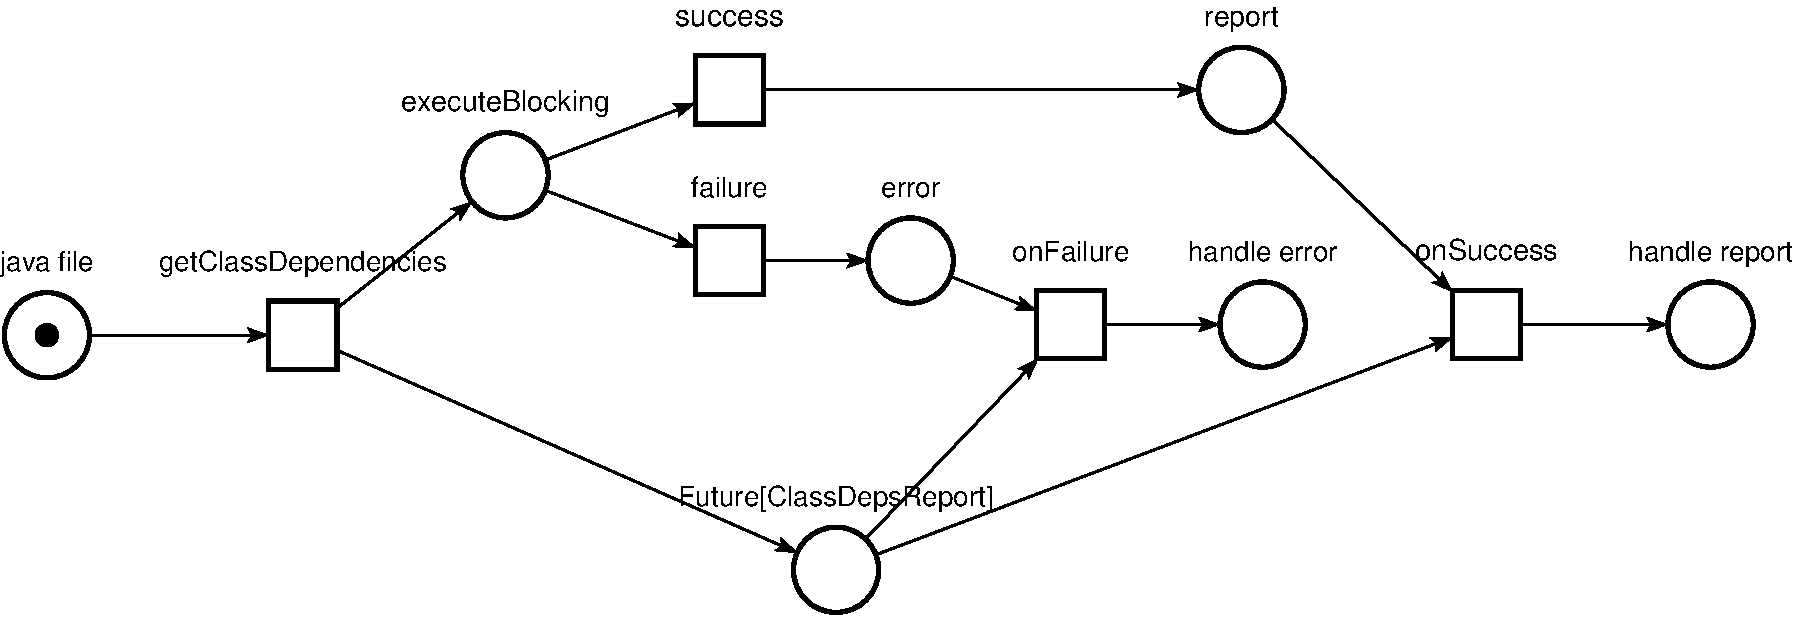
\includegraphics[width=\textwidth]{petri_nets_pdf/getClassDependencies.pdf}
    \caption{Rete di Petri per il flusso di esecuzione dell'analisi asincrona di una classe.}
    \label{fig:getClassDependencies}
    \end{figure}

    \begin{figure}[h!]
    \centering
    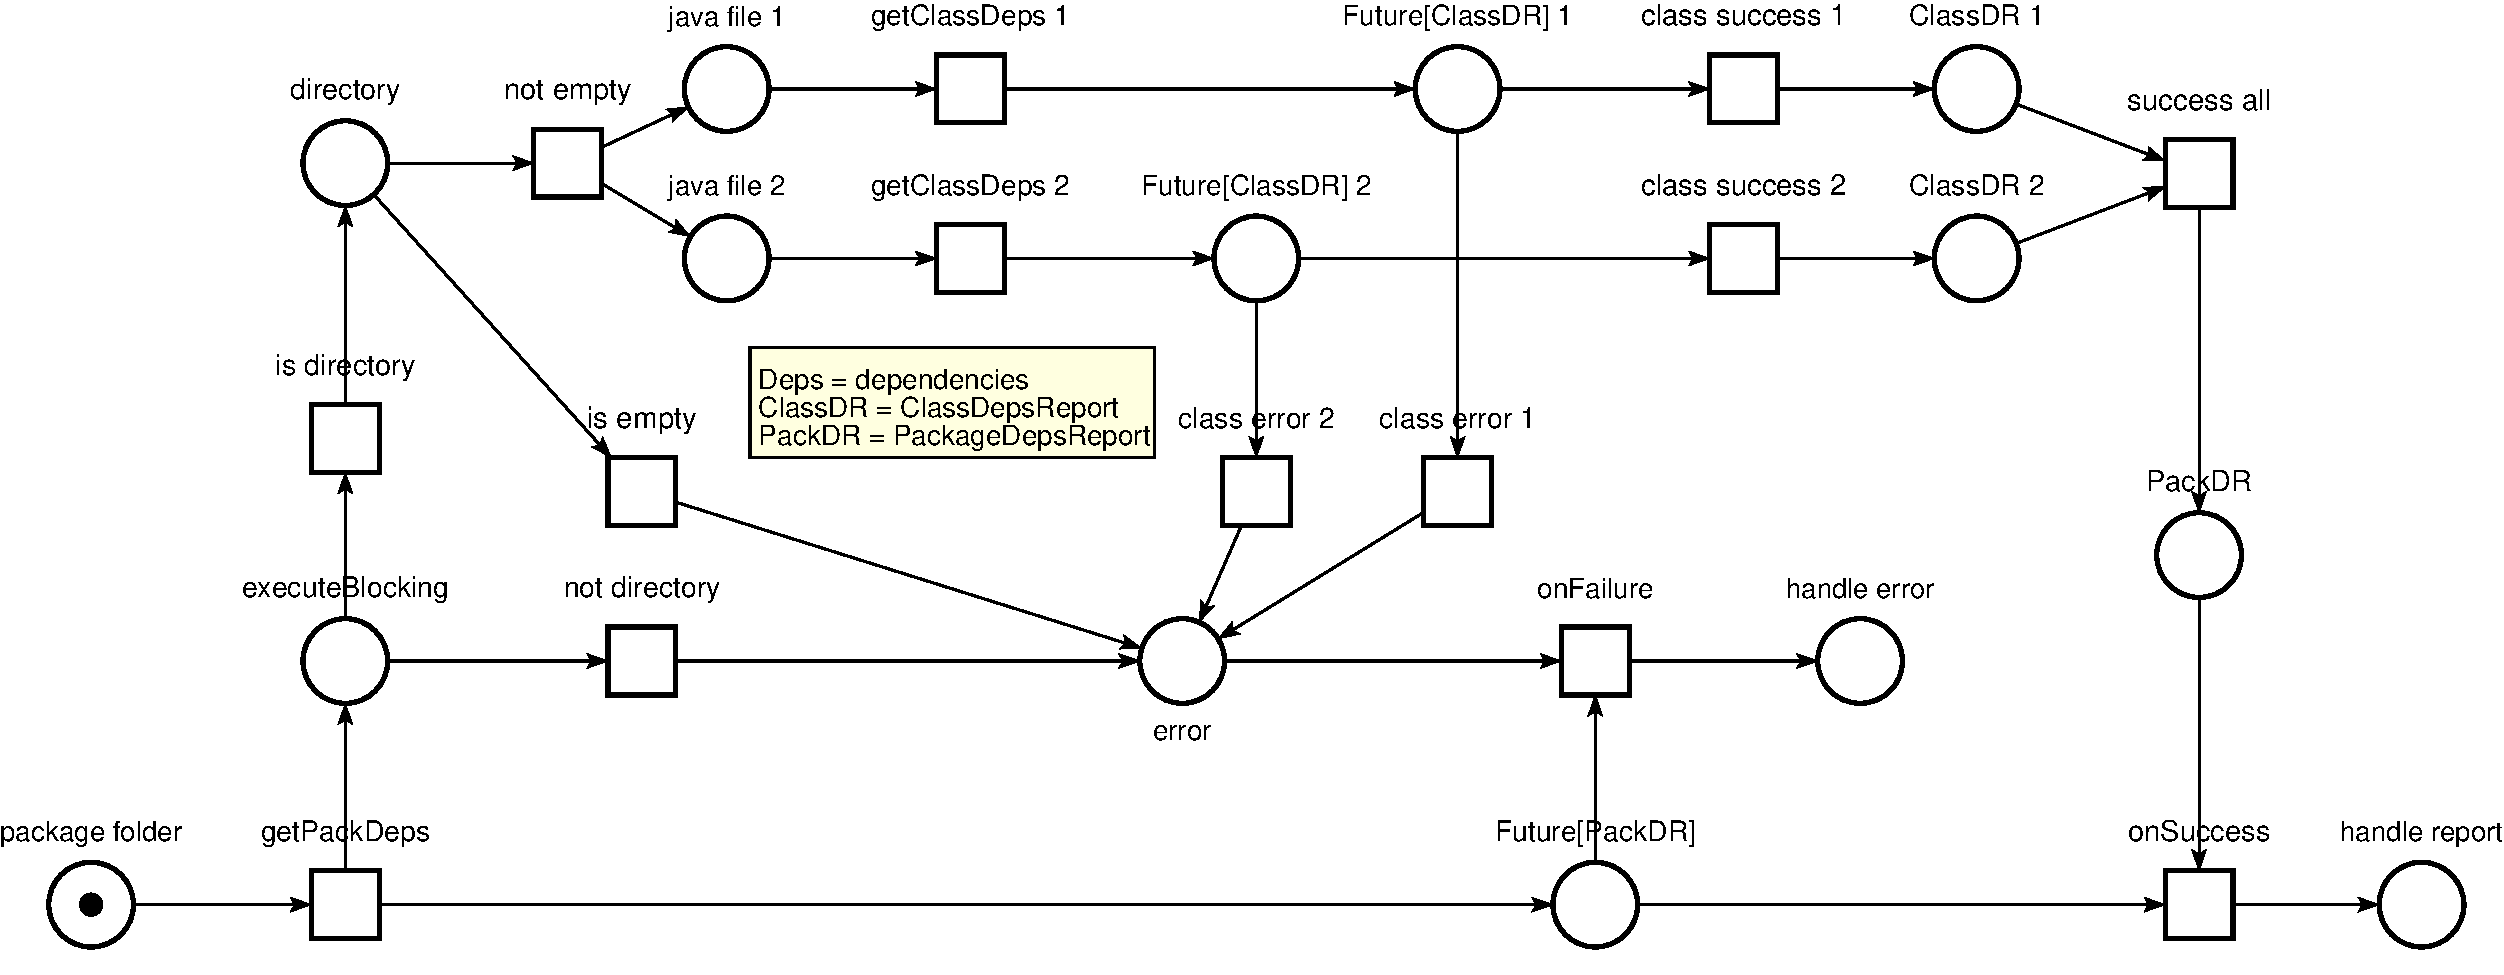
\includegraphics[width=\textwidth]{petri_nets_pdf/getPackageDependencies.pdf}
    \caption{Rete di Petri per il flusso di esecuzione dell'analisi asincrona di un package.}
    \label{fig:getPackageDependencies}
    \end{figure}

    \begin{figure}[h!]
    \centering
    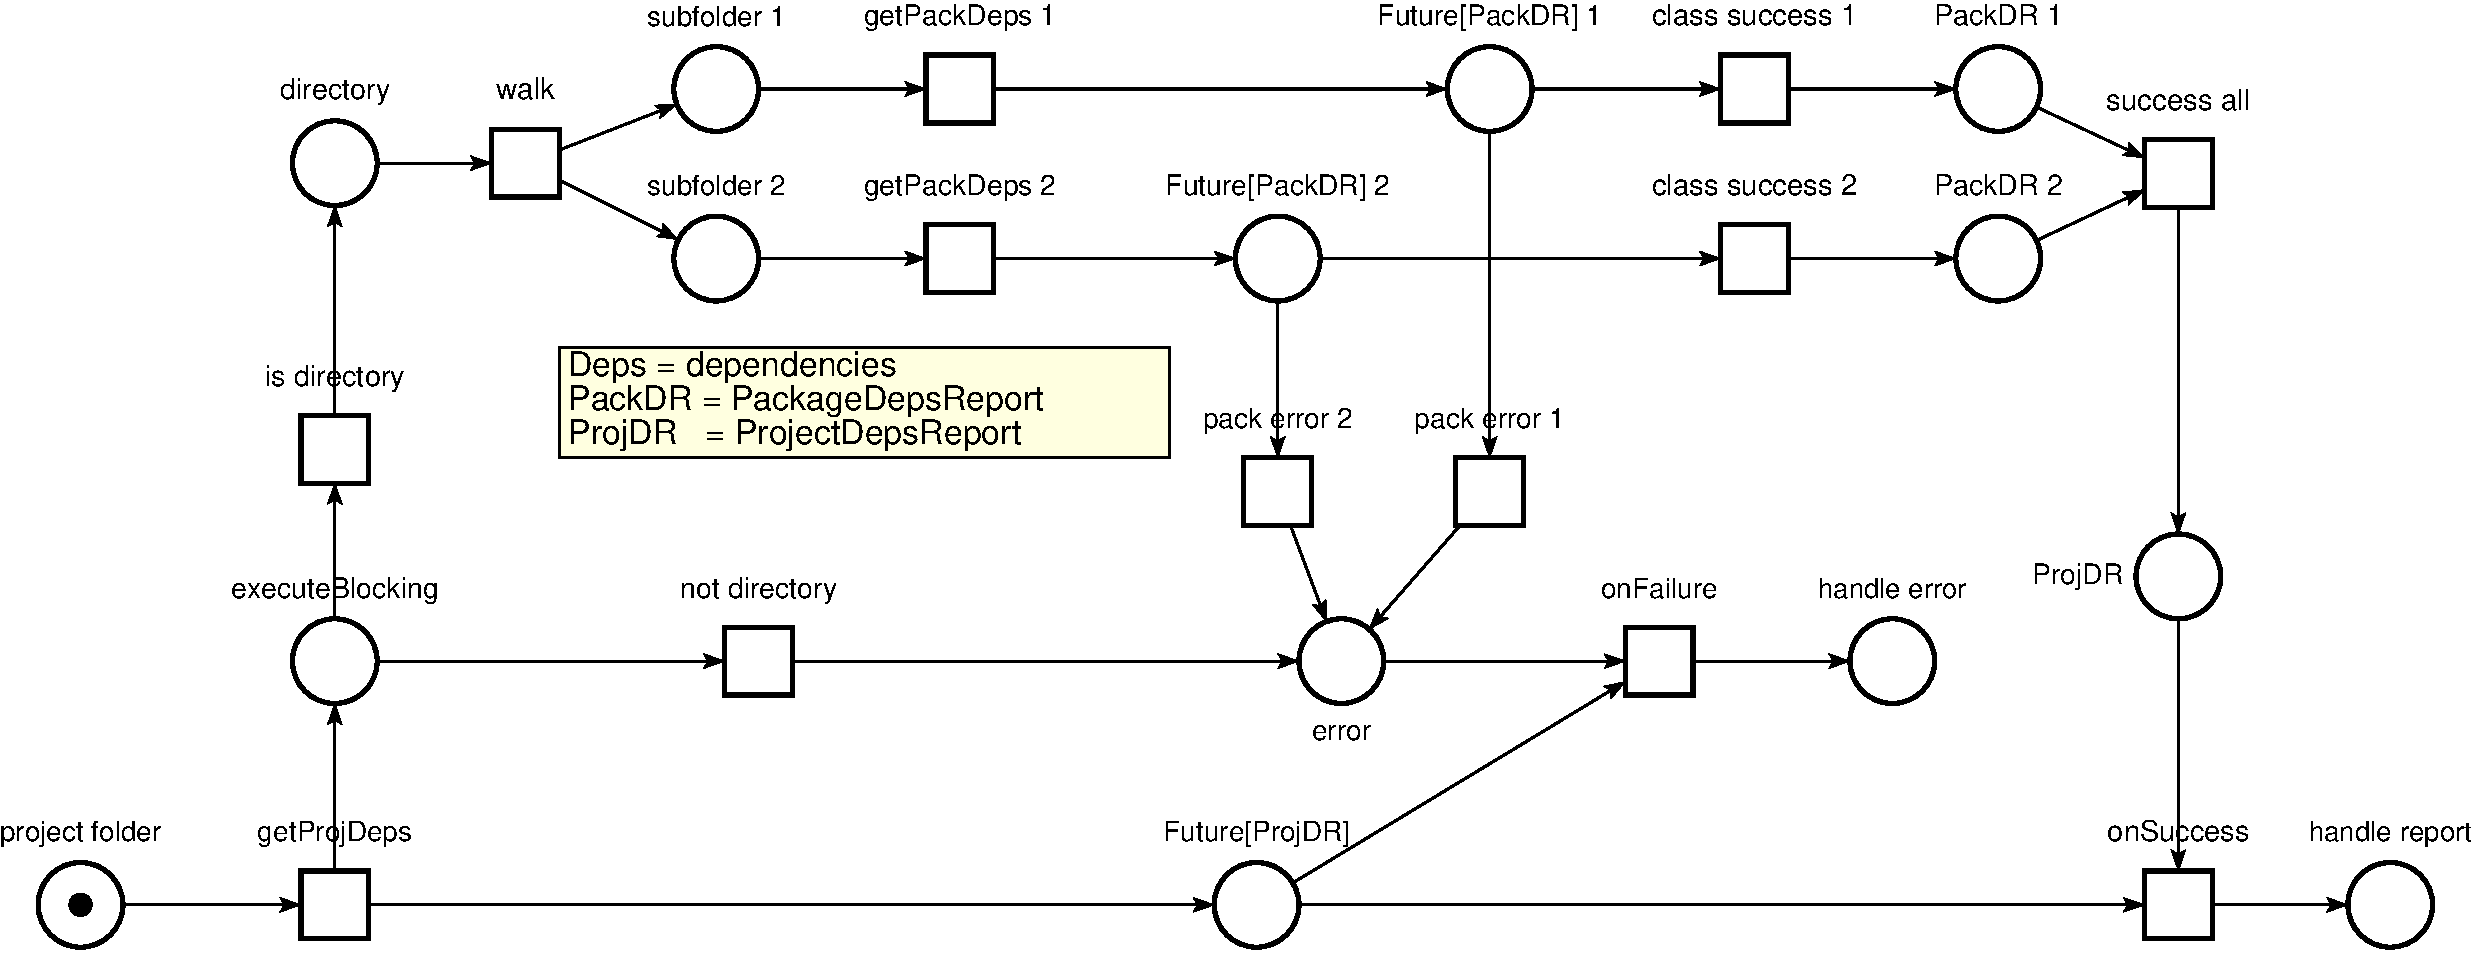
\includegraphics[width=\textwidth]{petri_nets_pdf/getProjectDependencies.pdf}
    \caption{Rete di Petri per il flusso di esecuzione dell'analisi asincrona di un progetto.}
    \label{fig:getProjectDependencies}
    \end{figure}

    \section{Punto 2 - Reactive GUI}
        Per lanciare l'applicazione si suggerisce il lancio di questo comando, in quanto abbiamo gestito le dipendenze con \texttt{Maven} e utilizzato le librerie esterne come \texttt{JavaFx} e \texttt{SmartGraph}:
    \begin{lstlisting}[style=bash, caption={Avvio dello script}]
        $ mvn clean javafx:run
    \end{lstlisting}

    \begin{figure}[h!]
    \centering
    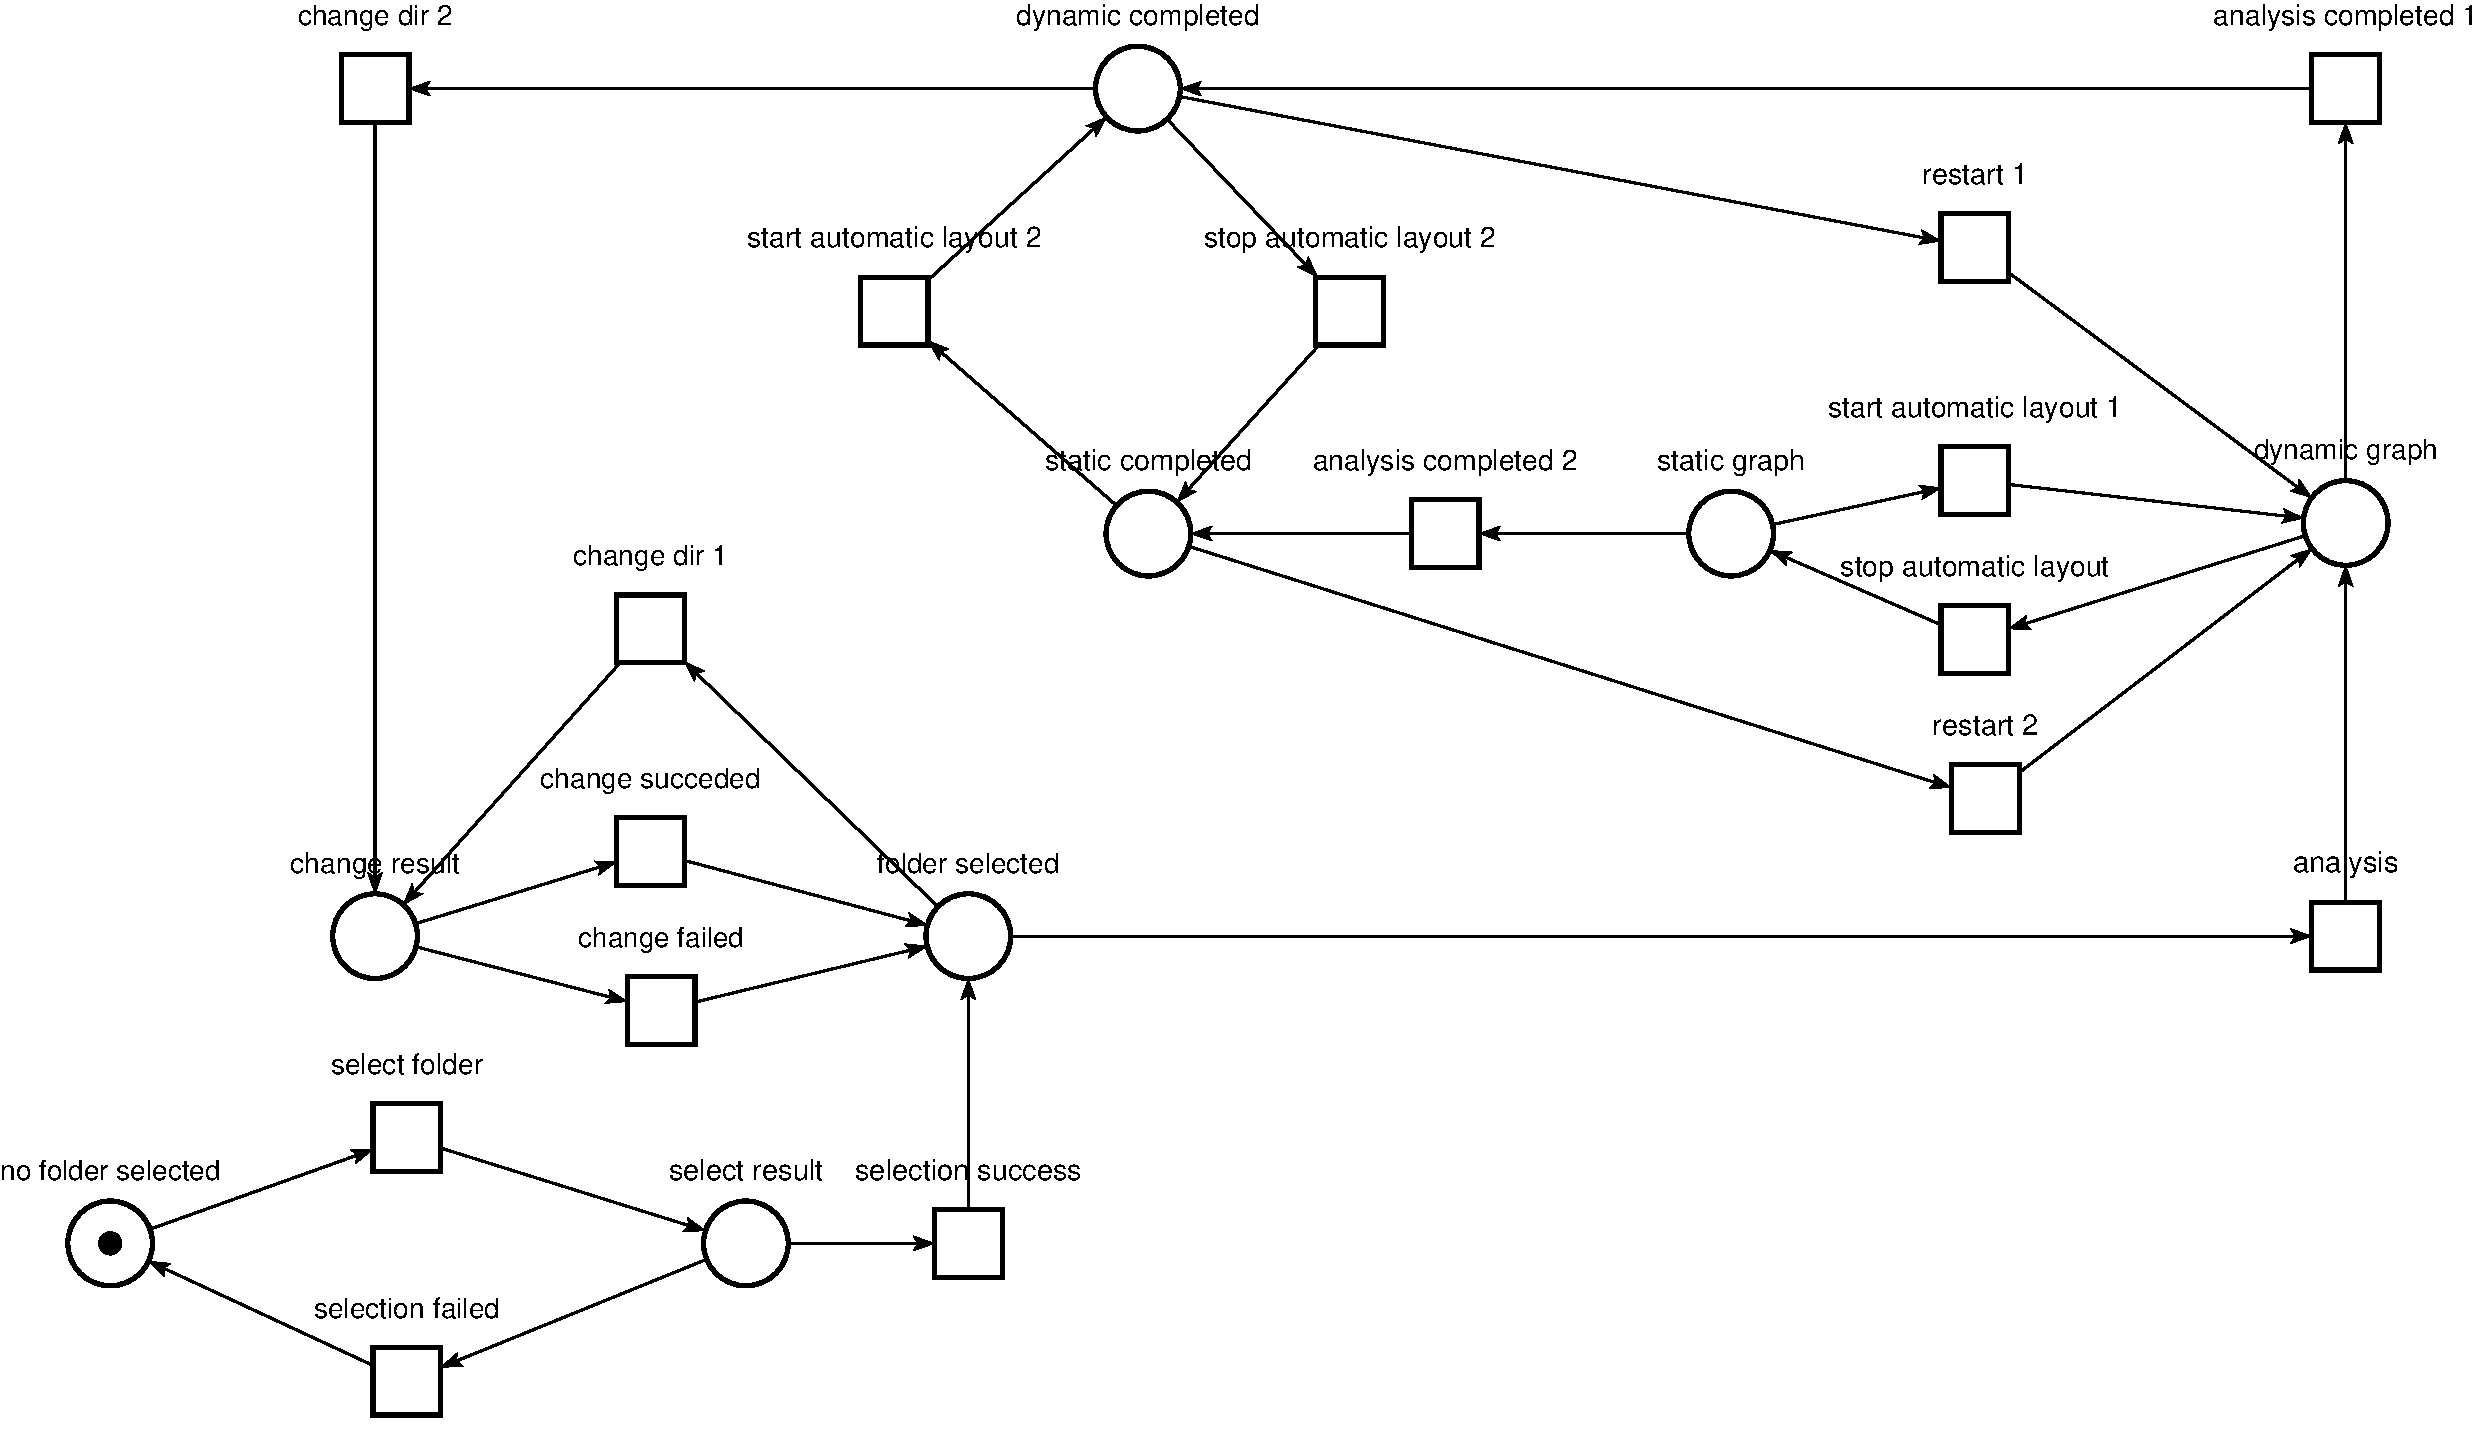
\includegraphics[width=\textwidth]{petri_nets_pdf/UI.pdf}
    \caption{Rete di Petri per il flusso di esecuzione con input dell'utente.}
    \label{fig:UI}
    \end{figure}

    \begin{figure}[h!]
    \centering
    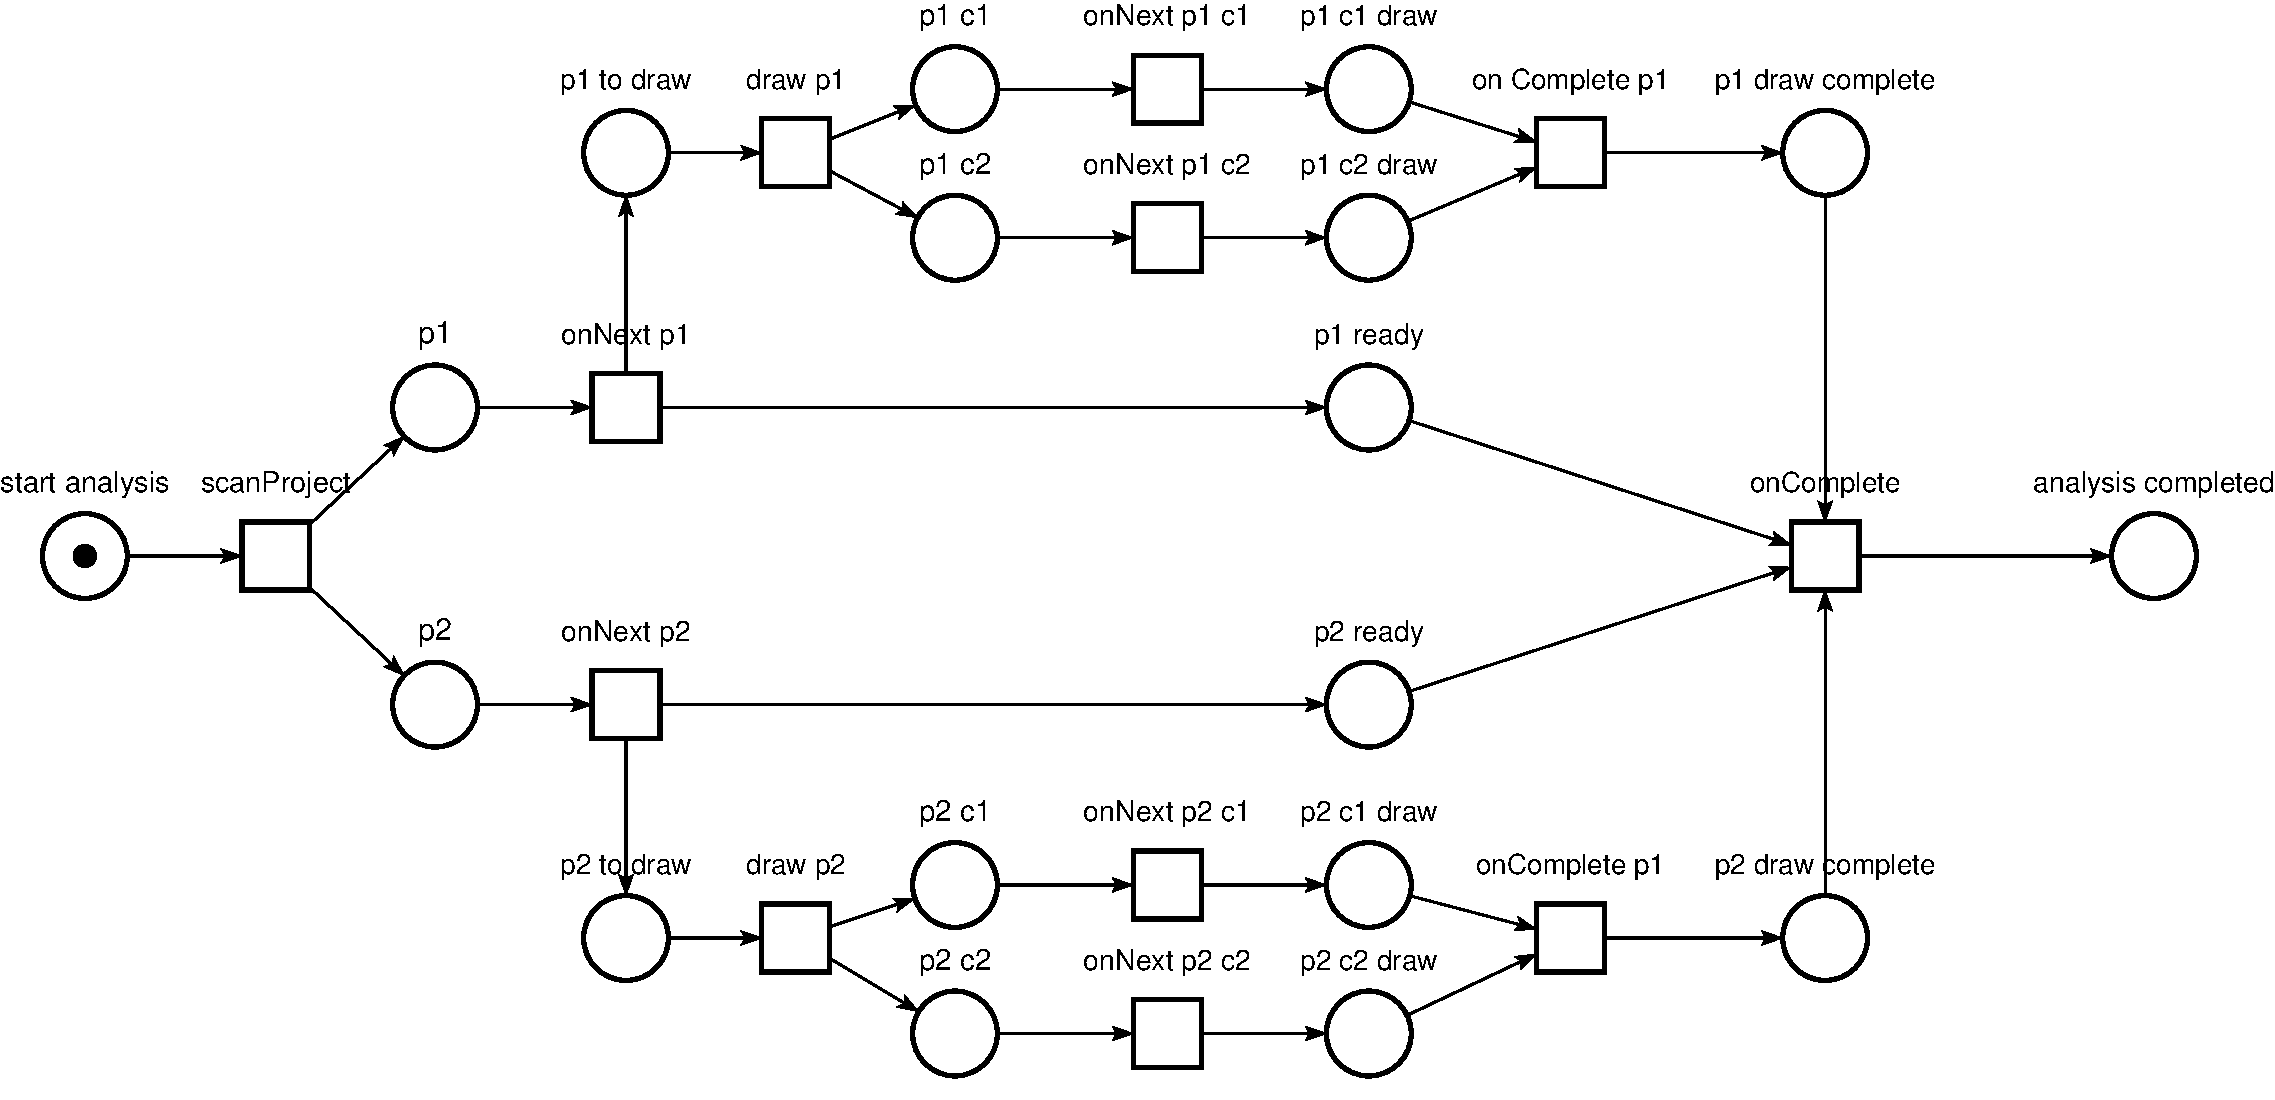
\includegraphics[width=\textwidth]{petri_nets_pdf/reactive_analysis.pdf}
    \caption{Rete di Petri per il flusso di esecuzione dell'analisi reattiva.}
    \label{fig:reactive_analysis}
    \end{figure}


    \begin{lstlisting}[style=java, caption={Metodo Java asincrono}]
public CompletableFuture<String> fetchDataAsync() {
    return CompletableFuture.supplyAsync(() -> fetchFromApi());
}
    \end{lstlisting}
    \begin{lstlisting}[style=scala, caption={Esempio reattivo in Scala}]
val source = Source(1 to 10)
source.mapAsync(2)(x => Future(x * 2)).runWith(Sink.foreach(println))
    \end{lstlisting}


\end{document}
